\PassOptionsToPackage{unicode=true}{hyperref} % options for packages loaded elsewhere
\PassOptionsToPackage{hyphens}{url}
%
\documentclass[]{article}
\usepackage{lmodern}
\usepackage{amssymb,amsmath}
\usepackage{ifxetex,ifluatex}
\usepackage{fixltx2e} % provides \textsubscript
\ifnum 0\ifxetex 1\fi\ifluatex 1\fi=0 % if pdftex
  \usepackage[T1]{fontenc}
  \usepackage[utf8]{inputenc}
  \usepackage{textcomp} % provides euro and other symbols
\else % if luatex or xelatex
  \usepackage{unicode-math}
  \defaultfontfeatures{Ligatures=TeX,Scale=MatchLowercase}
\fi
% use upquote if available, for straight quotes in verbatim environments
\IfFileExists{upquote.sty}{\usepackage{upquote}}{}
% use microtype if available
\IfFileExists{microtype.sty}{%
\usepackage[]{microtype}
\UseMicrotypeSet[protrusion]{basicmath} % disable protrusion for tt fonts
}{}
\IfFileExists{parskip.sty}{%
\usepackage{parskip}
}{% else
\setlength{\parindent}{0pt}
\setlength{\parskip}{6pt plus 2pt minus 1pt}
}
\usepackage{hyperref}
\hypersetup{
            pdftitle={STAT0011 ICA - Group 62},
            pdfborder={0 0 0},
            breaklinks=true}
\urlstyle{same}  % don't use monospace font for urls
\usepackage[margin=1in]{geometry}
\usepackage{color}
\usepackage{fancyvrb}
\newcommand{\VerbBar}{|}
\newcommand{\VERB}{\Verb[commandchars=\\\{\}]}
\DefineVerbatimEnvironment{Highlighting}{Verbatim}{commandchars=\\\{\}}
% Add ',fontsize=\small' for more characters per line
\usepackage{framed}
\definecolor{shadecolor}{RGB}{248,248,248}
\newenvironment{Shaded}{\begin{snugshade}}{\end{snugshade}}
\newcommand{\AlertTok}[1]{\textcolor[rgb]{0.94,0.16,0.16}{#1}}
\newcommand{\AnnotationTok}[1]{\textcolor[rgb]{0.56,0.35,0.01}{\textbf{\textit{#1}}}}
\newcommand{\AttributeTok}[1]{\textcolor[rgb]{0.77,0.63,0.00}{#1}}
\newcommand{\BaseNTok}[1]{\textcolor[rgb]{0.00,0.00,0.81}{#1}}
\newcommand{\BuiltInTok}[1]{#1}
\newcommand{\CharTok}[1]{\textcolor[rgb]{0.31,0.60,0.02}{#1}}
\newcommand{\CommentTok}[1]{\textcolor[rgb]{0.56,0.35,0.01}{\textit{#1}}}
\newcommand{\CommentVarTok}[1]{\textcolor[rgb]{0.56,0.35,0.01}{\textbf{\textit{#1}}}}
\newcommand{\ConstantTok}[1]{\textcolor[rgb]{0.00,0.00,0.00}{#1}}
\newcommand{\ControlFlowTok}[1]{\textcolor[rgb]{0.13,0.29,0.53}{\textbf{#1}}}
\newcommand{\DataTypeTok}[1]{\textcolor[rgb]{0.13,0.29,0.53}{#1}}
\newcommand{\DecValTok}[1]{\textcolor[rgb]{0.00,0.00,0.81}{#1}}
\newcommand{\DocumentationTok}[1]{\textcolor[rgb]{0.56,0.35,0.01}{\textbf{\textit{#1}}}}
\newcommand{\ErrorTok}[1]{\textcolor[rgb]{0.64,0.00,0.00}{\textbf{#1}}}
\newcommand{\ExtensionTok}[1]{#1}
\newcommand{\FloatTok}[1]{\textcolor[rgb]{0.00,0.00,0.81}{#1}}
\newcommand{\FunctionTok}[1]{\textcolor[rgb]{0.00,0.00,0.00}{#1}}
\newcommand{\ImportTok}[1]{#1}
\newcommand{\InformationTok}[1]{\textcolor[rgb]{0.56,0.35,0.01}{\textbf{\textit{#1}}}}
\newcommand{\KeywordTok}[1]{\textcolor[rgb]{0.13,0.29,0.53}{\textbf{#1}}}
\newcommand{\NormalTok}[1]{#1}
\newcommand{\OperatorTok}[1]{\textcolor[rgb]{0.81,0.36,0.00}{\textbf{#1}}}
\newcommand{\OtherTok}[1]{\textcolor[rgb]{0.56,0.35,0.01}{#1}}
\newcommand{\PreprocessorTok}[1]{\textcolor[rgb]{0.56,0.35,0.01}{\textit{#1}}}
\newcommand{\RegionMarkerTok}[1]{#1}
\newcommand{\SpecialCharTok}[1]{\textcolor[rgb]{0.00,0.00,0.00}{#1}}
\newcommand{\SpecialStringTok}[1]{\textcolor[rgb]{0.31,0.60,0.02}{#1}}
\newcommand{\StringTok}[1]{\textcolor[rgb]{0.31,0.60,0.02}{#1}}
\newcommand{\VariableTok}[1]{\textcolor[rgb]{0.00,0.00,0.00}{#1}}
\newcommand{\VerbatimStringTok}[1]{\textcolor[rgb]{0.31,0.60,0.02}{#1}}
\newcommand{\WarningTok}[1]{\textcolor[rgb]{0.56,0.35,0.01}{\textbf{\textit{#1}}}}
\usepackage{longtable,booktabs}
% Fix footnotes in tables (requires footnote package)
\IfFileExists{footnote.sty}{\usepackage{footnote}\makesavenoteenv{longtable}}{}
\usepackage{graphicx,grffile}
\makeatletter
\def\maxwidth{\ifdim\Gin@nat@width>\linewidth\linewidth\else\Gin@nat@width\fi}
\def\maxheight{\ifdim\Gin@nat@height>\textheight\textheight\else\Gin@nat@height\fi}
\makeatother
% Scale images if necessary, so that they will not overflow the page
% margins by default, and it is still possible to overwrite the defaults
% using explicit options in \includegraphics[width, height, ...]{}
\setkeys{Gin}{width=\maxwidth,height=\maxheight,keepaspectratio}
\setlength{\emergencystretch}{3em}  % prevent overfull lines
\providecommand{\tightlist}{%
  \setlength{\itemsep}{0pt}\setlength{\parskip}{0pt}}
\setcounter{secnumdepth}{0}
% Redefines (sub)paragraphs to behave more like sections
\ifx\paragraph\undefined\else
\let\oldparagraph\paragraph
\renewcommand{\paragraph}[1]{\oldparagraph{#1}\mbox{}}
\fi
\ifx\subparagraph\undefined\else
\let\oldsubparagraph\subparagraph
\renewcommand{\subparagraph}[1]{\oldsubparagraph{#1}\mbox{}}
\fi

% set default figure placement to htbp
\makeatletter
\def\fps@figure{htbp}
\makeatother


\title{STAT0011 ICA - Group 62}
\author{}
\date{\vspace{-2.5em}}

\begin{document}
\maketitle
\begin{abstract}
The aim of this report is to measure the market risk of a portfolio for
the selected financial assets, to provide level of risk for such
relative investment and to decide whether or not to invest in
consequence.
\end{abstract}

\hypertarget{a-exploratory-analysis}{%
\subsection{(a) Exploratory Analysis}\label{a-exploratory-analysis}}

Throughout this report, FTSE100 and S\&P500 served as two selected stock
indices. We obtain their weekly data from 3 Jan 2000 to 25 Dec 2020 and
calculate their log returns respectively, using the following code.
Here, `coredata' function is used to extract the observations for
returns, and stripe off their corresponding time index for simplicity.

\begin{Shaded}
\begin{Highlighting}[]
\CommentTok{##### Question (a)}
\CommentTok{### Download historical weekly prices for S&P500 and FTSE100 from 2000-01-03 to 2020-12-26}
\NormalTok{SP500 <-}\StringTok{ }\KeywordTok{get.hist.quote}\NormalTok{(}\DataTypeTok{instrument =} \StringTok{"^GSPC"}\NormalTok{, }\DataTypeTok{start =} \StringTok{"2000-01-03"}\NormalTok{,}
                         \DataTypeTok{end =} \StringTok{"2020-12-26"}\NormalTok{, }\DataTypeTok{compression =} \StringTok{"w"}\NormalTok{, }\DataTypeTok{quote=}\StringTok{"Close"}\NormalTok{)}
\NormalTok{FTSE100 <-}\StringTok{ }\KeywordTok{get.hist.quote}\NormalTok{(}\DataTypeTok{instrument =} \StringTok{"^FTSE"}\NormalTok{, }\DataTypeTok{start =} \StringTok{"2000-01-03"}\NormalTok{,}
                          \DataTypeTok{end =} \StringTok{"2020-12-26"}\NormalTok{, }\DataTypeTok{compression =} \StringTok{"w"}\NormalTok{, }\DataTypeTok{quote=}\StringTok{"Close"}\NormalTok{)}

\CommentTok{### Calculate the weekly log-returns and extract the values from the 'zoo' series}
\NormalTok{ret.SP500.tmp <-}\StringTok{ }\KeywordTok{diff}\NormalTok{(}\KeywordTok{log}\NormalTok{(SP500), }\DataTypeTok{lag =} \DecValTok{1}\NormalTok{)}
\NormalTok{ret.FTSE100.tmp <-}\StringTok{ }\KeywordTok{diff}\NormalTok{(}\KeywordTok{log}\NormalTok{(FTSE100), }\DataTypeTok{lag =} \DecValTok{1}\NormalTok{)}
\NormalTok{ret.SP500 <-}\StringTok{ }\KeywordTok{coredata}\NormalTok{(ret.SP500.tmp)}
\NormalTok{ret.FTSE100 <-}\StringTok{ }\KeywordTok{coredata}\NormalTok{(ret.FTSE100.tmp)}
\end{Highlighting}
\end{Shaded}

The figures shown below give an overview of the fluctuations of
log-returns on S\&P500 and FTSE100 during 2000-2020.

\begin{figure}

{\centering \includegraphics{Group_62_Report_files/figure-latex/Overview-1} 

}

\caption{Weekly log-returns for S\&P500 and FTSE100, 2000-2020}\label{fig:Overview}
\end{figure}

The summary table including mean, median, standard deviation, minimum,
maximum, skewness and kurtosis is as follows:

\begin{longtable}[]{@{}llllllrr@{}}
\caption{S\&P500 and FTSE100 weekly log-return summary
table}\tabularnewline
\toprule
Stock & Mean & Median & Sd & Min & Max & Skewness &
Kurtosis\tabularnewline
\midrule
\endfirsthead
\toprule
Stock & Mean & Median & Sd & Min & Max & Skewness &
Kurtosis\tabularnewline
\midrule
\endhead
S\&P 500 & 0.086\% & 0.217\% & 2.537\% & -20.084\% & 11.424\% & -0.963 &
7.784\tabularnewline
FTSE 100 & -0.000\% & 0.191\% & 2.482\% & -23.632\% & 12.583\% & -1.267
& 12.386\tabularnewline
\bottomrule
\end{longtable}

\newpage

From the above table we see that the kurtosis for S\&P500 and FTSE100
are 7.784 and 12.386 respectively, which are larger than Normal
distribution with kurtosis = 3, indicating that the log-returns have a
heavier tail than Normal distribution. The skewness are -0.963 and
-1.267 respectively, which means the distributions of log-returns are
asymmetric and the negative values imply that the distributions are left
skewed. We then check the normality visually by plotting their relative
plots.

\begin{figure}

{\centering \includegraphics{Group_62_Report_files/figure-latex/Normality-1} 

}

\caption{Density plots and Q-Q plots for S\&P500 (Left) and FTSE100 (Right)}\label{fig:Normality}
\end{figure}

According to the density plot, the deviation from the theoretical bell
curve seems not too significant but there appears to be a heavier tail
which coincides with our previous findings. For qqplot, which shows the
distribution of the data against the expected normal distribution, not
all quantile points lie along the theoretical red line, especially near
the tails.

Then, to test whether the log returns follow a normal distribution
formally, a series of tests can be performed. Both Shapiro test and
Jarque Bera test give very low p values, which reject the null
hypothesis of normality, potentially because they are time varying.
Hence, we conclude that there is less evidence to support the normality
assumption.

\newpage

\begin{Shaded}
\begin{Highlighting}[]
\CommentTok{# Normality tests}
\KeywordTok{shapiro.test}\NormalTok{(ret.SP500); }\KeywordTok{shapiro.test}\NormalTok{(ret.FTSE100)}
\end{Highlighting}
\end{Shaded}

\begin{verbatim}
## 
##  Shapiro-Wilk normality test
## 
## data:  ret.SP500
## W = 0.91467, p-value < 2.2e-16
\end{verbatim}

\begin{verbatim}
## 
##  Shapiro-Wilk normality test
## 
## data:  ret.FTSE100
## W = 0.90195, p-value < 2.2e-16
\end{verbatim}

\begin{Shaded}
\begin{Highlighting}[]
\KeywordTok{jarque.bera.test}\NormalTok{(ret.SP500); }\KeywordTok{jarque.bera.test}\NormalTok{(ret.FTSE100)}
\end{Highlighting}
\end{Shaded}

\begin{verbatim}
## 
##  Jarque Bera Test
## 
## data:  ret.SP500
## X-squared = 2945.3, df = 2, p-value < 2.2e-16
\end{verbatim}

\begin{verbatim}
## 
##  Jarque Bera Test
## 
## data:  ret.FTSE100
## X-squared = 7318.4, df = 2, p-value < 2.2e-16
\end{verbatim}

\hypertarget{b-value-at-risk-historical-simulation-approach}{%
\subsection{(b) Value at Risk: Historical Simulation
approach}\label{b-value-at-risk-historical-simulation-approach}}

We construct an equally weighted portfolio as required, using
log-returns of S\&P500 and FTSE100. After that, we calculate the Value
at Risk, which is the maximum expected loss over a given period at 95\%
and 99\% confidence level, respectively. Code and results are listed
below:

\begin{Shaded}
\begin{Highlighting}[]
\CommentTok{##### Question (b)}
\CommentTok{### Estimate VaR using Historical Simulation approach}

\NormalTok{Pof <-}\StringTok{ }\KeywordTok{cbind}\NormalTok{(ret.SP500, ret.FTSE100)                          }\CommentTok{# Combine two log-returns }
\NormalTok{w <-}\StringTok{ }\KeywordTok{matrix}\NormalTok{(}\KeywordTok{c}\NormalTok{(}\FloatTok{0.5}\NormalTok{, }\FloatTok{0.5}\NormalTok{))                                      }\CommentTok{# Equal portfolio weights}

\NormalTok{ret.Pof <-}\StringTok{ }\KeywordTok{log}\NormalTok{(}\DecValTok{1}\OperatorTok{+}\NormalTok{((}\KeywordTok{exp}\NormalTok{(Pof[,}\DecValTok{1}\NormalTok{])}\OperatorTok{-}\DecValTok{1}\NormalTok{)}\OperatorTok{+}\NormalTok{(}\KeywordTok{exp}\NormalTok{(Pof[,}\DecValTok{2}\NormalTok{])}\OperatorTok{-}\DecValTok{1}\NormalTok{))}\OperatorTok{*}\NormalTok{(}\DecValTok{1}\OperatorTok{/}\DecValTok{2}\NormalTok{))   }\CommentTok{# Portfolio log-returns}
\NormalTok{ret.Pof.s <-}\StringTok{ }\KeywordTok{sort}\NormalTok{(ret.Pof)                                    }\CommentTok{# Sort the log-returns}

\NormalTok{VaR.HS}\FloatTok{.99}\NormalTok{ <-}\StringTok{ }\OperatorTok{-}\KeywordTok{quantile}\NormalTok{(ret.Pof.s, }\FloatTok{0.01}\NormalTok{)                       }\CommentTok{# Calculate 99% VaR using HS}
\NormalTok{VaR.HS}\FloatTok{.95}\NormalTok{ <-}\StringTok{ }\OperatorTok{-}\KeywordTok{quantile}\NormalTok{(ret.Pof.s, }\FloatTok{0.05}\NormalTok{)                       }\CommentTok{# Calculate 95% VaR using HS}

\KeywordTok{cat}\NormalTok{(}\StringTok{"The 99% 1-week VaR of the portfolio using Historical Simulation approach is "}\NormalTok{,}
    \KeywordTok{percent}\NormalTok{(VaR.HS}\FloatTok{.99}\NormalTok{), }\StringTok{"."}\NormalTok{, }\DataTypeTok{sep =} \StringTok{""}\NormalTok{)}
\end{Highlighting}
\end{Shaded}

\begin{verbatim}
## The 99% 1-week VaR of the portfolio using Historical Simulation approach is 7.283%.
\end{verbatim}

\begin{Shaded}
\begin{Highlighting}[]
\KeywordTok{cat}\NormalTok{(}\StringTok{"The 95% 1-week VaR of the portfolio using Historical Simulation approach is "}\NormalTok{,}
    \KeywordTok{percent}\NormalTok{(VaR.HS}\FloatTok{.95}\NormalTok{), }\StringTok{"."}\NormalTok{, }\DataTypeTok{sep =} \StringTok{""}\NormalTok{)}
\end{Highlighting}
\end{Shaded}

\begin{verbatim}
## The 95% 1-week VaR of the portfolio using Historical Simulation approach is 3.574%.
\end{verbatim}

Historical Simulation approach does not introduce parameters and is
purely based on the past observed returns, which make it intuitive and
can be easily interpreted for individual traders. Besides, when working
with portfolio, HS can capture nonlinear dependence by directly using
the portfolio returns without analysing each asset in the portfolio.
However, HS does have a few drawbacks. Firstly, it relies on the quality
of the historical dataset completely, thus the accuracy of HS can only
be as good as historic data. Here, we calculate VaR by including market
data for the past 20 years, which may not be reflective of the same
market today. For instance, the financial crisis during 2007-2009 can
have a downward influence on returns. Secondly, it cannot adapt with the
changes of market structure, such as the federal reserve rate hike,
which causes 2000 Dot-com Bubble and 2007 housing Bubble. Other
macroeconomic events such as Brexit and its extending, the China-US
trade war and more recently, the coronavirus pandemic may affect the
stock market as well. (Figures available in Appex.B) Especially given
the fact that many firms within FTSE100 make a large fraction of their
profits in US dollars. (We can try to solve this either by using most
recent data or by giving more weight on recent observations, which
consequently leads to exacerbation of standard error.)

\hypertarget{c-parametric-approach}{%
\subsection{(c) Parametric approach}\label{c-parametric-approach}}

Under the assumption that the joint distribution of log-returns is
bivariate normal, we calculate the VaR for the portfolio using
parametric approach: \[
VaR_{\alpha,P} = \Phi^{-1}(\alpha)\sigma_P - \mu_P, \ \ \text{where} \ \ \sigma_P^2 = \mathbf{w' \Sigma w},\  \mu_P = \mathbf{w' \mu}. 
\] The expected return is estimated using the sample mean and the
standard deviation is estimated using the sample covariance matrix. Code
and results are listed below:

\begin{Shaded}
\begin{Highlighting}[]
\CommentTok{##### Question (c)}
\CommentTok{### Estimate VaR using parametric approach based on normality assumption}
\NormalTok{sigma <-}\StringTok{ }\KeywordTok{sqrt}\NormalTok{(}\KeywordTok{t}\NormalTok{(w) }\OperatorTok\StringTok{ }\KeywordTok{cov}\NormalTok{(Pof) }\OperatorTok\StringTok{ }\NormalTok{w)      }\CommentTok{# Estimate portfolio volatility}
\NormalTok{mu <-}\StringTok{ }\KeywordTok{t}\NormalTok{(w) }\OperatorTok\StringTok{ }\KeywordTok{apply}\NormalTok{(Pof, }\DecValTok{2}\NormalTok{, }\StringTok{"mean"}\NormalTok{)        }\CommentTok{# Estimate portfolio mean}

\NormalTok{VaR.Para}\FloatTok{.99}\NormalTok{ <-}\StringTok{ }\KeywordTok{as.numeric}\NormalTok{(}\OperatorTok{-}\NormalTok{sigma }\OperatorTok{*}\StringTok{ }\KeywordTok{qnorm}\NormalTok{(}\FloatTok{0.01}\NormalTok{) }\OperatorTok{-}\StringTok{ }\NormalTok{mu)   }\CommentTok{# 99% VaR using Parametric}
\NormalTok{VaR.Para}\FloatTok{.95}\NormalTok{ <-}\StringTok{ }\KeywordTok{as.numeric}\NormalTok{(}\OperatorTok{-}\NormalTok{sigma }\OperatorTok{*}\StringTok{ }\KeywordTok{qnorm}\NormalTok{(}\FloatTok{0.05}\NormalTok{) }\OperatorTok{-}\StringTok{ }\NormalTok{mu)   }\CommentTok{# 95% VaR using Parametric}

\KeywordTok{cat}\NormalTok{(}\StringTok{"The 99% 1-week VaR of the portfolio using parametric approach is "}\NormalTok{,}
    \KeywordTok{percent}\NormalTok{(VaR.Para}\FloatTok{.99}\NormalTok{), }\StringTok{"."}\NormalTok{, }\DataTypeTok{sep =} \StringTok{""}\NormalTok{)}
\end{Highlighting}
\end{Shaded}

\begin{verbatim}
## The 99% 1-week VaR of the portfolio using parametric approach is 5.494%.
\end{verbatim}

\begin{Shaded}
\begin{Highlighting}[]
\KeywordTok{cat}\NormalTok{(}\StringTok{"The 95% 1-week VaR of the portfolio using parametric approach is "}\NormalTok{,}
    \KeywordTok{percent}\NormalTok{(VaR.Para}\FloatTok{.95}\NormalTok{), }\StringTok{"."}\NormalTok{, }\DataTypeTok{sep =} \StringTok{""}\NormalTok{)}
\end{Highlighting}
\end{Shaded}

\begin{verbatim}
## The 95% 1-week VaR of the portfolio using parametric approach is 3.872%.
\end{verbatim}

\begin{Shaded}
\begin{Highlighting}[]
\KeywordTok{skewness}\NormalTok{(ret.Pof)[}\DecValTok{1}\NormalTok{]}
\end{Highlighting}
\end{Shaded}

\begin{verbatim}
## [1] -1.084855
\end{verbatim}

\begin{Shaded}
\begin{Highlighting}[]
\KeywordTok{kurtosis}\NormalTok{(ret.Pof)[}\DecValTok{1}\NormalTok{]}
\end{Highlighting}
\end{Shaded}

\begin{verbatim}
## [1] 10.17415
\end{verbatim}

\begin{figure}

{\centering \includegraphics[width=0.8\linewidth]{Group_62_Report_files/figure-latex/unnamed-chunk-6-1} 

}

\caption{Density plot for the portfolio}\label{fig:unnamed-chunk-6}
\end{figure}

The primary advantage of parametric approach is that it is fast and
simple for computation. By assuming normality, we automatically know
where the worst 5\% and 1\% locate. Since the parameter estimation
includes volatility updates, there is no need to assume that the
distribution of returns is stationary over time. However, it relies
heavily on the assumption of normal distribution, and it is widely
believed that the returns of the market have larger tails than the true
normal distribution and the volatility is time varying. After
calculation, we have a skewness of -1.085, which differs from the
theoretical zero value for normal distribution, and the kurtosis result
(greater than 3, rule of thumb) also verifies this. For highly skewed
distributions, the effectiveness of Central Limit Theorem may be
eliminated.

\hypertarget{d-copula-based-monte-carlo-approach}{%
\subsection{(d) Copula-based Monte Carlo
approach}\label{d-copula-based-monte-carlo-approach}}

Based on copula theory, we have the following procedure for Monte Carlo
simulation approach to estimate portfolio VaR:

\begin{enumerate}
\def\labelenumi{\arabic{enumi}.}
\tightlist
\item
  Identify two AR models by observing ACF and PACF for the log-returns
  of S\&P 500 and FTSE 100, respectively. Also, we need to check if a
  GARCH model is necessary (and if the series is indeed i.i.d) by
  observing ACF for the squared log-returns. No MA models will be
  considered in this case.\\
\item
  Fit the models found in Step 1.\\
\item
  Evaluate the fitted models using ACF plots for the residuals and the
  squared residuals, followed by a Ljung--Box test to confirm the series
  is uncorrelated.\\
\item
  Transform the residuals to copula data `u' \(\sim U(0, 1)\) using
  corresponding conditional distribution functions (CDF) and check if
  the generated `u' is uniformly distributed using Kolmogorov-Smirnov
  test. (Step 1-4 is the Box-Jenkins approach to fit a model.)\\
\item
  Select an appropriate bivariate copula family given `u' and estimate
  the corresponding parameters using function `BiCopSelect'.\\
\item
  Simulate 10,000 bivariate observations given the copula selected in
  Step 5.\\
\item
  Invert the simulated random bivariate observations using the inverse
  CDF of \(N(0, 1)\). (We assume the marginal models are N(0,1),
  completely ignoring the results above.)\\
\item
  Compute the simulated portfolio returns and then the VaR.
\end{enumerate}

First, we have the following ACF and PACF plots:

\newpage

\begin{figure}

{\centering \includegraphics{Group_62_Report_files/figure-latex/unnamed-chunk-7-1} 

}

\caption{ACF and PACF plots for S\&P500 and FTSE100}\label{fig:unnamed-chunk-7}
\end{figure}

For S\&P500, it appears to be no ACF and PACF and the spike of PACF at
lag 1 and 4 are not significant. Hence, an AR(0) model is selected for
S\&P500, which is also suggested by `auto.arima' with criterion BIC. For
FTSE100, the spike of PACF at lag 3 is considerable and accordingly, the
ACF decays at lag 3 simultaneously. Hence, we would like to choose AR(3)
for FTSE100. After fitting the chosen models, there seem to be no ACF
for both residuals and squared residuals indicating good fits. Here are
the Ljung--Box test results for the chosen models:

\begin{longtable}[]{@{}lrr@{}}
\caption{VaR summary table for all three methods}\tabularnewline
\toprule
Residuals & Original & Squared\tabularnewline
\midrule
\endfirsthead
\toprule
Residuals & Original & Squared\tabularnewline
\midrule
\endhead
S\&P500 & 0.6114237 & 0.4163981\tabularnewline
FTSE100 & 0.3599072 & 0.1595850\tabularnewline
\bottomrule
\end{longtable}

We see that all the p-values are quite large, thus we cannot reject the
null hypothesis that there is no autocorrelation, that is, now the
residuals seem independent. To get a smallest possible
Kolmogorov-Smirnov test p-value, we tried the combinations of every
potential AR models and marginal distributions with corresponding CDF.
It truned out that for S\&P500, when choosing Student's t-distribution
with mean = 0, sd = 1, the KS test p-value reaches the peak, 0.1622,
which indicates significant evidence that the copula data is drawn from
standard uniform distribution; for FTSE100, when choosing Normal
distribution with mean = 0, sd = 1, the KS test p-value reaches the
peak, 0.0048. Although the p-value is too small to validate the
uniformity assumption, we have tried every possibilities and the model
is the best one we can find for AR(p)-GARCH(1,1) with different
`cond.dist'. It probably can be improved by introducing other GARCH
extensions such as TGARCH and APARCH. Below are the probability integral
transform histograms for the copula data.

\begin{figure}

{\centering \includegraphics{Group_62_Report_files/figure-latex/unnamed-chunk-10-1} 

}

\caption{PIT Histograms for S\&P500 and FTSE100}\label{fig:unnamed-chunk-10}
\end{figure}

Next, we use `BiCopSelect' to select an appropriate bivariate copula
using criterion AIC after testing the independence of the copula data.
The copula selected is Student-t copula with two parameters being 0.75
and 12.4 respectively, and the dependence measurement Kendall's tau is
0.54. The dependence structure of the copula can be described by the
linear correlation coefficient. It has tail dependence but it imposes
symmetry in both tails. Then we simulate random observations given the
Student-t copula with a seed set to achieve same results. Assuming both
marginal distributions are \(N(0, 1)\), we can easily simulate a series
of pseudo log-returns and compute the VaR. The results are listed below:
(Full code available in Appx.A)

\begin{Shaded}
\begin{Highlighting}[]
\CommentTok{### Step 8: Value-at-Risk uisng Monte Carlo simulation}
\NormalTok{portsim <-}\StringTok{ }\KeywordTok{matrix}\NormalTok{(}\DecValTok{0}\NormalTok{, }\DataTypeTok{nrow =}\NormalTok{ N, }\DataTypeTok{ncol =} \DecValTok{1}\NormalTok{)}
\NormalTok{varsim <-}\StringTok{ }\KeywordTok{matrix}\NormalTok{(}\DecValTok{0}\NormalTok{, }\DataTypeTok{nrow =} \DecValTok{1}\NormalTok{, }\DataTypeTok{ncol =} \DecValTok{2}\NormalTok{)}
\NormalTok{portsim=}\KeywordTok{log}\NormalTok{(}\DecValTok{1}\OperatorTok{+}\NormalTok{((}\KeywordTok{exp}\NormalTok{(y1simulated)}\OperatorTok{-}\DecValTok{1}\NormalTok{)}\OperatorTok{+}\NormalTok{(}\KeywordTok{exp}\NormalTok{(y2simulated)}\OperatorTok{-}\DecValTok{1}\NormalTok{))}\OperatorTok{*}\NormalTok{(}\DecValTok{1}\OperatorTok{/}\DecValTok{2}\NormalTok{))}
\NormalTok{VaR.MC}\FloatTok{.99}\NormalTok{ <-}\StringTok{ }\OperatorTok{-}\KeywordTok{quantile}\NormalTok{(portsim, }\FloatTok{0.01}\NormalTok{)}
\NormalTok{VaR.MC}\FloatTok{.95}\NormalTok{ <-}\StringTok{ }\OperatorTok{-}\KeywordTok{quantile}\NormalTok{(portsim, }\FloatTok{0.05}\NormalTok{)}
\KeywordTok{cat}\NormalTok{(}\StringTok{"The 99% 1-week VaR of the portfolio using Monto Carlo approach is "}\NormalTok{,}
    \KeywordTok{percent}\NormalTok{(VaR.MC}\FloatTok{.99}\NormalTok{), }\StringTok{"."}\NormalTok{, }\DataTypeTok{sep =} \StringTok{""}\NormalTok{)}
\end{Highlighting}
\end{Shaded}

\begin{verbatim}
## The 99% 1-week VaR of the portfolio using Monto Carlo approach is 215.072%.
\end{verbatim}

\begin{Shaded}
\begin{Highlighting}[]
\KeywordTok{cat}\NormalTok{(}\StringTok{"The 95% 1-week VaR of the portfolio using Monto Carlo approach is "}\NormalTok{,}
    \KeywordTok{percent}\NormalTok{(VaR.MC}\FloatTok{.95}\NormalTok{), }\StringTok{"."}\NormalTok{, }\DataTypeTok{sep =} \StringTok{""}\NormalTok{)}
\end{Highlighting}
\end{Shaded}

\begin{verbatim}
## The 95% 1-week VaR of the portfolio using Monto Carlo approach is 147.758%.
\end{verbatim}

Monte Carlo methods essentially estimates the uncertainty in a model,
and it can be applied to various types of portfolios. It is able to
capture non-linearity and thus works well in non-linear models, along
with complex pricing patterns. It is not bounded by the historical data,
and can be extended to longer horizons, which provides a broader
opportunity on observing possible outcomes, hence gives a clearer view
to traders upon deciding an investment. Theoretically, as the number of
the simulations tends to infinity, the MC estimates converges to specfic
values. Compared with other approaches, it also shows probabilistic
results, i.e.~how likely each outcome is. By accounting for a wider
range of risks, it sacrifices the easiness while computing as it
requires higher computing skill, which is an apparent drawback, along
with its consumption on time. The joint distribution assumption and
parameters selection are vital, hence demanding extra carefulness in
model selection. By introducing copula theory, we do not need to make
any assumptions for the joint distribution and in this case it allows us
to decompose a 2-demensional joint distribution into two marginal
distributions and a bivariate copula function (Step 4-5), which makes
the following simulations a lot easier. However, for convienience, here
we assume that both marginal models for both log-returns are \(N(0, 1)\)
instead of using the estimated distributions in Step 4 (the actual
variance cannot be as large as 1), thus the estimated VaR looks
ridiculous and unreasonable. If we reduced the estimated variance or use
the estimated distribution, the VaR would be more reasonable. Besides,
contrast to reality, it may not create extreme values of returns as it
may not reflect fat tails accurately.

\hypertarget{e-var-comparison}{%
\subsection{(e) VaR comparison}\label{e-var-comparison}}

Here we have the summary table of VaR for all three methods:

\begin{longtable}[]{@{}llll@{}}
\caption{VaR summary table for all three methods}\tabularnewline
\toprule
VaR & HS.approach & Parametric.approach &
Monto.Carlo.approach\tabularnewline
\midrule
\endfirsthead
\toprule
VaR & HS.approach & Parametric.approach &
Monto.Carlo.approach\tabularnewline
\midrule
\endhead
95\% VaR & 3.574\% & 3.872\% & 147.758\%\tabularnewline
99\% VaR & 7.283\% & 5.494\% & 215.072\%\tabularnewline
\bottomrule
\end{longtable}

Normally, Monte Carlo approach would be the choice with priority, as it
generates random trials and is flexible in terms of covering various
types of portfolio. Here, we have assumed that the marginal models for
log returns follow a standard normal distribution as required, which
volatiles the true standard deviation, hence result in a dramatic
difference compared with other approaches. We choose to use the
parametric approach as an alternative, as it gives a relatively
reasonable and consistent result. It is worth noticing that VaR does not
measure the worst-case loss, traders should always bear in mind this
limitation while investing.

\vspace{3cm}

\hypertarget{references}{%
\section{References}\label{references}}

\hypertarget{refs}{}
\leavevmode\hypertarget{ref-DanielssonJon2011FRFT}{}%
Danielsson, Jon, and Jaon Danaielsson. 2011. \emph{Financial Risk
Forecasting: The Theory and Practice of Forecasting Market Risk with
Implementation in R and Matlab}. Vol. 590. Wiley Finance Series.
Hoboken: John Wiley \& Sons, Incorporated.

\leavevmode\hypertarget{ref-Ravi}{}%
Madapati, Ravi. 2003. ``A Ceo's Guide to Value at Risk Models.''
\url{http://janroman.dhis.org/finance/VaR/rm.pdf}.

\leavevmode\hypertarget{ref-Michael}{}%
Msika, Michael. 2020. ``Four Years After the Vote, Brexit Still Haunts
Uk Stocks.''
\url{https://www.bloomberg.com/news/articles/2020-06-24/four-years-after-the-referendum-brexit-still-haunts-u-k-stocks?sref=4aM5ycm9}.

\leavevmode\hypertarget{ref-Wipplinger}{}%
Wipplinger, Evert. 2007. ``Philippe Jorion: Value at Risk -- the New
Benchmark for Managing Financial Risk: 3rd Edition, Isbn 0-07-146495-6,
Mcgraw--Hill, 2007, 602~Pages, Approx. 120 Chf (Hardcover).''
\emph{Financial Markets and Portfolio Management} 21 (3). Boston:
Springer US: 397--98.

\leavevmode\hypertarget{ref-2628584}{}%
Xu, Chao, and Huigeng Chen. 2012. ``Measuring Portfolio Value at Risk.''
\url{http://lup.lub.lu.se/student-papers/record/2628584}.

\newpage

\hypertarget{appendix-a-all-code-for-this-ica}{%
\section{Appendix A: All code for this
ICA}\label{appendix-a-all-code-for-this-ica}}

\begin{Shaded}
\begin{Highlighting}[]
\NormalTok{knitr}\OperatorTok{::}\NormalTok{opts_chunk}\OperatorTok{$}\KeywordTok{set}\NormalTok{(}\DataTypeTok{echo =} \OtherTok{FALSE}\NormalTok{)}
\KeywordTok{library}\NormalTok{(tseries) }
\KeywordTok{library}\NormalTok{(knitr)}
\KeywordTok{library}\NormalTok{(moments)}
\KeywordTok{library}\NormalTok{(scales)}
\KeywordTok{library}\NormalTok{(zoo)}
\KeywordTok{library}\NormalTok{(fGarch)}
\KeywordTok{library}\NormalTok{(KScorrect)}
\KeywordTok{library}\NormalTok{(ADGofTest)}
\KeywordTok{library}\NormalTok{(VineCopula)}
\KeywordTok{library}\NormalTok{(forecast)}
\KeywordTok{library}\NormalTok{(here)}

\CommentTok{### Format a number as percentage}
\NormalTok{percent <-}\StringTok{ }\ControlFlowTok{function}\NormalTok{(x, }\DataTypeTok{digits =} \DecValTok{3}\NormalTok{, }\DataTypeTok{format =} \StringTok{"f"}\NormalTok{, ...) \{}
  \KeywordTok{paste0}\NormalTok{(}\KeywordTok{formatC}\NormalTok{(}\DecValTok{100} \OperatorTok{*}\StringTok{ }\NormalTok{x, }\DataTypeTok{format =}\NormalTok{ format, }\DataTypeTok{digits =}\NormalTok{ digits, ...), }\StringTok{"%"}\NormalTok{)}
\NormalTok{\}}

\KeywordTok{options}\NormalTok{(}\StringTok{"getSymbols.warning4.0"}\NormalTok{=}\OtherTok{FALSE}\NormalTok{)}

\CommentTok{##### Question (a)}
\CommentTok{### Download historical weekly prices for S&P500 and FTSE100 from 2000-01-03 to 2020-12-26}
\NormalTok{SP500 <-}\StringTok{ }\KeywordTok{get.hist.quote}\NormalTok{(}\DataTypeTok{instrument =} \StringTok{"^GSPC"}\NormalTok{, }\DataTypeTok{start =} \StringTok{"2000-01-03"}\NormalTok{,}
                         \DataTypeTok{end =} \StringTok{"2020-12-26"}\NormalTok{, }\DataTypeTok{compression =} \StringTok{"w"}\NormalTok{, }\DataTypeTok{quote=}\StringTok{"Close"}\NormalTok{)}
\NormalTok{FTSE100 <-}\StringTok{ }\KeywordTok{get.hist.quote}\NormalTok{(}\DataTypeTok{instrument =} \StringTok{"^FTSE"}\NormalTok{, }\DataTypeTok{start =} \StringTok{"2000-01-03"}\NormalTok{,}
                          \DataTypeTok{end =} \StringTok{"2020-12-26"}\NormalTok{, }\DataTypeTok{compression =} \StringTok{"w"}\NormalTok{, }\DataTypeTok{quote=}\StringTok{"Close"}\NormalTok{)}

\CommentTok{### Calculate the weekly log-returns and extract the values from the 'zoo' series}
\NormalTok{ret.SP500.tmp <-}\StringTok{ }\KeywordTok{diff}\NormalTok{(}\KeywordTok{log}\NormalTok{(SP500), }\DataTypeTok{lag =} \DecValTok{1}\NormalTok{)}
\NormalTok{ret.FTSE100.tmp <-}\StringTok{ }\KeywordTok{diff}\NormalTok{(}\KeywordTok{log}\NormalTok{(FTSE100), }\DataTypeTok{lag =} \DecValTok{1}\NormalTok{)}
\NormalTok{ret.SP500 <-}\StringTok{ }\KeywordTok{coredata}\NormalTok{(ret.SP500.tmp)}
\NormalTok{ret.FTSE100 <-}\StringTok{ }\KeywordTok{coredata}\NormalTok{(ret.FTSE100.tmp)}

\CommentTok{### Time series plots for log-returns}
\KeywordTok{par}\NormalTok{(}\DataTypeTok{mfrow =} \KeywordTok{c}\NormalTok{(}\DecValTok{1}\NormalTok{, }\DecValTok{2}\NormalTok{))}
\KeywordTok{plot}\NormalTok{(ret.SP500.tmp, }\DataTypeTok{cex.lab =} \FloatTok{0.6}\NormalTok{, }\DataTypeTok{cex.axis =} \FloatTok{0.6}\NormalTok{, }\DataTypeTok{xlab =} \StringTok{""}\NormalTok{, }\DataTypeTok{ylab =} \StringTok{"SP500 log-returns"}\NormalTok{)}
\KeywordTok{plot}\NormalTok{(ret.FTSE100.tmp, }\DataTypeTok{cex.lab =} \FloatTok{0.6}\NormalTok{, }\DataTypeTok{cex.axis =} \FloatTok{0.6}\NormalTok{, }\DataTypeTok{xlab =} \StringTok{""}\NormalTok{, }\DataTypeTok{ylab =} \StringTok{"FTSE100 log-returns"}\NormalTok{)}

\CommentTok{### Print the summary table}
\NormalTok{Stock <-}\StringTok{ }\KeywordTok{c}\NormalTok{(}\StringTok{'S&P 500'}\NormalTok{, }\StringTok{'FTSE 100'}\NormalTok{)}
\NormalTok{ret.mean <-}\StringTok{ }\KeywordTok{c}\NormalTok{(}\KeywordTok{percent}\NormalTok{(}\KeywordTok{mean}\NormalTok{(ret.SP500), }\DecValTok{3}\NormalTok{), }\KeywordTok{percent}\NormalTok{(}\KeywordTok{mean}\NormalTok{(ret.FTSE100), }\DecValTok{3}\NormalTok{))}
\NormalTok{ret.median <-}\StringTok{ }\KeywordTok{c}\NormalTok{(}\KeywordTok{percent}\NormalTok{(}\KeywordTok{median}\NormalTok{(ret.SP500)), }\KeywordTok{percent}\NormalTok{(}\KeywordTok{median}\NormalTok{(ret.FTSE100)))}
\NormalTok{ret.sd <-}\StringTok{ }\KeywordTok{c}\NormalTok{(}\KeywordTok{percent}\NormalTok{(}\KeywordTok{sd}\NormalTok{(ret.SP500)), }\KeywordTok{percent}\NormalTok{(}\KeywordTok{sd}\NormalTok{(ret.FTSE100)))}
\NormalTok{ret.min <-}\StringTok{ }\KeywordTok{c}\NormalTok{(}\KeywordTok{percent}\NormalTok{(}\KeywordTok{min}\NormalTok{(ret.SP500)), }\KeywordTok{percent}\NormalTok{(}\KeywordTok{min}\NormalTok{(ret.FTSE100)))}
\NormalTok{ret.max <-}\StringTok{ }\KeywordTok{c}\NormalTok{(}\KeywordTok{percent}\NormalTok{(}\KeywordTok{max}\NormalTok{(ret.SP500)), }\KeywordTok{percent}\NormalTok{(}\KeywordTok{max}\NormalTok{(ret.FTSE100)))}
\NormalTok{ret.skewness <-}\StringTok{ }\KeywordTok{c}\NormalTok{(}\KeywordTok{round}\NormalTok{(}\KeywordTok{skewness}\NormalTok{(ret.SP500), }\DecValTok{3}\NormalTok{), }\KeywordTok{round}\NormalTok{(}\KeywordTok{skewness}\NormalTok{(ret.FTSE100), }\DecValTok{3}\NormalTok{))}
\NormalTok{ret.kurtosis <-}\StringTok{ }\KeywordTok{c}\NormalTok{(}\KeywordTok{round}\NormalTok{(}\KeywordTok{kurtosis}\NormalTok{(ret.SP500), }\DecValTok{3}\NormalTok{), }\KeywordTok{round}\NormalTok{(}\KeywordTok{kurtosis}\NormalTok{(ret.FTSE100), }\DecValTok{3}\NormalTok{))}
\CommentTok{# ret.p <- c(percent(jarque.bera.test(ret.SP500)$p.value, digits = 4),}
\CommentTok{#            percent(jarque.bera.test(ret.FTSE100)$p.value, digits = 4))}

\NormalTok{ret.summary <-}\StringTok{ }\KeywordTok{data.frame}\NormalTok{(Stock, }\DataTypeTok{Mean =}\NormalTok{ ret.mean, }\DataTypeTok{Median =}\NormalTok{ ret.median, }\DataTypeTok{Sd =}\NormalTok{ ret.sd,}
                          \DataTypeTok{Min =}\NormalTok{ ret.min, }\DataTypeTok{Max =}\NormalTok{ ret.max, }\DataTypeTok{Skewness =}\NormalTok{ ret.skewness,}
                          \DataTypeTok{Kurtosis =}\NormalTok{ ret.kurtosis)}

\KeywordTok{kable}\NormalTok{(ret.summary, }\DataTypeTok{caption =} \StringTok{"S&P500 and FTSE100 weekly log-return summary table"}\NormalTok{)}

\KeywordTok{par}\NormalTok{(}\DataTypeTok{mfrow =} \KeywordTok{c}\NormalTok{(}\DecValTok{2}\NormalTok{, }\DecValTok{2}\NormalTok{))}

\CommentTok{### Density plots for log-returns}
\KeywordTok{plot}\NormalTok{(}\KeywordTok{density}\NormalTok{(ret.SP500), }\DataTypeTok{main =} \StringTok{"Density plot for S&P500"}\NormalTok{)}
\KeywordTok{plot}\NormalTok{(}\KeywordTok{density}\NormalTok{(ret.FTSE100), }\DataTypeTok{main =} \StringTok{"Density plot for FTSE100"}\NormalTok{)}

\CommentTok{### Q-Q plots for log-returns}
\KeywordTok{qqnorm}\NormalTok{(ret.SP500, }\DataTypeTok{cex =} \FloatTok{0.4}\NormalTok{, }\DataTypeTok{main =} \StringTok{"Q-Q plot for S&P500"}\NormalTok{)}
\KeywordTok{qqline}\NormalTok{(ret.SP500, }\DataTypeTok{lty =} \DecValTok{2}\NormalTok{, }\DataTypeTok{col =} \StringTok{"red"}\NormalTok{)}
\KeywordTok{qqnorm}\NormalTok{(ret.FTSE100, }\DataTypeTok{cex =} \FloatTok{0.4}\NormalTok{, }\DataTypeTok{main =} \StringTok{"Q-Q plot for FTSE100"}\NormalTok{)}
\KeywordTok{qqline}\NormalTok{(ret.FTSE100, }\DataTypeTok{lty =} \DecValTok{2}\NormalTok{, }\DataTypeTok{col =} \StringTok{"red"}\NormalTok{)}

\CommentTok{# Normality tests}
\KeywordTok{shapiro.test}\NormalTok{(ret.SP500); }\KeywordTok{shapiro.test}\NormalTok{(ret.FTSE100)}
\KeywordTok{jarque.bera.test}\NormalTok{(ret.SP500); }\KeywordTok{jarque.bera.test}\NormalTok{(ret.FTSE100)}

\CommentTok{##### Question (b)}
\CommentTok{### Estimate VaR using Historical Simulation approach}

\NormalTok{Pof <-}\StringTok{ }\KeywordTok{cbind}\NormalTok{(ret.SP500, ret.FTSE100)                          }\CommentTok{# Combine two log-returns }
\NormalTok{w <-}\StringTok{ }\KeywordTok{matrix}\NormalTok{(}\KeywordTok{c}\NormalTok{(}\FloatTok{0.5}\NormalTok{, }\FloatTok{0.5}\NormalTok{))                                      }\CommentTok{# Equal portfolio weights}

\NormalTok{ret.Pof <-}\StringTok{ }\KeywordTok{log}\NormalTok{(}\DecValTok{1}\OperatorTok{+}\NormalTok{((}\KeywordTok{exp}\NormalTok{(Pof[,}\DecValTok{1}\NormalTok{])}\OperatorTok{-}\DecValTok{1}\NormalTok{)}\OperatorTok{+}\NormalTok{(}\KeywordTok{exp}\NormalTok{(Pof[,}\DecValTok{2}\NormalTok{])}\OperatorTok{-}\DecValTok{1}\NormalTok{))}\OperatorTok{*}\NormalTok{(}\DecValTok{1}\OperatorTok{/}\DecValTok{2}\NormalTok{))   }\CommentTok{# Portfolio log-returns}
\NormalTok{ret.Pof.s <-}\StringTok{ }\KeywordTok{sort}\NormalTok{(ret.Pof)                                    }\CommentTok{# Sort the log-returns}

\NormalTok{VaR.HS}\FloatTok{.99}\NormalTok{ <-}\StringTok{ }\OperatorTok{-}\KeywordTok{quantile}\NormalTok{(ret.Pof.s, }\FloatTok{0.01}\NormalTok{)                       }\CommentTok{# Calculate 99% VaR using HS}
\NormalTok{VaR.HS}\FloatTok{.95}\NormalTok{ <-}\StringTok{ }\OperatorTok{-}\KeywordTok{quantile}\NormalTok{(ret.Pof.s, }\FloatTok{0.05}\NormalTok{)                       }\CommentTok{# Calculate 95% VaR using HS}

\KeywordTok{cat}\NormalTok{(}\StringTok{"The 99% 1-week VaR of the portfolio using Historical Simulation approach is "}\NormalTok{,}
    \KeywordTok{percent}\NormalTok{(VaR.HS}\FloatTok{.99}\NormalTok{), }\StringTok{"."}\NormalTok{, }\DataTypeTok{sep =} \StringTok{""}\NormalTok{)}
\KeywordTok{cat}\NormalTok{(}\StringTok{"The 95% 1-week VaR of the portfolio using Historical Simulation approach is "}\NormalTok{,}
    \KeywordTok{percent}\NormalTok{(VaR.HS}\FloatTok{.95}\NormalTok{), }\StringTok{"."}\NormalTok{, }\DataTypeTok{sep =} \StringTok{""}\NormalTok{)}

\CommentTok{##### Question (c)}
\CommentTok{### Estimate VaR using parametric approach based on normality assumption}
\NormalTok{sigma <-}\StringTok{ }\KeywordTok{sqrt}\NormalTok{(}\KeywordTok{t}\NormalTok{(w) }\OperatorTok\StringTok{ }\KeywordTok{cov}\NormalTok{(Pof) }\OperatorTok\StringTok{ }\NormalTok{w)      }\CommentTok{# Estimate portfolio volatility}
\NormalTok{mu <-}\StringTok{ }\KeywordTok{t}\NormalTok{(w) }\OperatorTok\StringTok{ }\KeywordTok{apply}\NormalTok{(Pof, }\DecValTok{2}\NormalTok{, }\StringTok{"mean"}\NormalTok{)        }\CommentTok{# Estimate portfolio mean}

\NormalTok{VaR.Para}\FloatTok{.99}\NormalTok{ <-}\StringTok{ }\KeywordTok{as.numeric}\NormalTok{(}\OperatorTok{-}\NormalTok{sigma }\OperatorTok{*}\StringTok{ }\KeywordTok{qnorm}\NormalTok{(}\FloatTok{0.01}\NormalTok{) }\OperatorTok{-}\StringTok{ }\NormalTok{mu)   }\CommentTok{# 99% VaR using Parametric}
\NormalTok{VaR.Para}\FloatTok{.95}\NormalTok{ <-}\StringTok{ }\KeywordTok{as.numeric}\NormalTok{(}\OperatorTok{-}\NormalTok{sigma }\OperatorTok{*}\StringTok{ }\KeywordTok{qnorm}\NormalTok{(}\FloatTok{0.05}\NormalTok{) }\OperatorTok{-}\StringTok{ }\NormalTok{mu)   }\CommentTok{# 95% VaR using Parametric}

\KeywordTok{cat}\NormalTok{(}\StringTok{"The 99% 1-week VaR of the portfolio using parametric approach is "}\NormalTok{,}
    \KeywordTok{percent}\NormalTok{(VaR.Para}\FloatTok{.99}\NormalTok{), }\StringTok{"."}\NormalTok{, }\DataTypeTok{sep =} \StringTok{""}\NormalTok{)}
\KeywordTok{cat}\NormalTok{(}\StringTok{"The 95% 1-week VaR of the portfolio using parametric approach is "}\NormalTok{,}
    \KeywordTok{percent}\NormalTok{(VaR.Para}\FloatTok{.95}\NormalTok{), }\StringTok{"."}\NormalTok{, }\DataTypeTok{sep =} \StringTok{""}\NormalTok{)}

\KeywordTok{skewness}\NormalTok{(ret.Pof)[}\DecValTok{1}\NormalTok{]}
\KeywordTok{kurtosis}\NormalTok{(ret.Pof)[}\DecValTok{1}\NormalTok{]}
\KeywordTok{plot}\NormalTok{(}\KeywordTok{density}\NormalTok{(ret.Pof), }\DataTypeTok{main =} \StringTok{""}\NormalTok{)}

\CommentTok{##### Question (d)}
\CommentTok{### Building AR models: the Box - Jenkins approach}
\CommentTok{### Step 1: Identification}
\KeywordTok{par}\NormalTok{(}\DataTypeTok{mfrow=}\KeywordTok{c}\NormalTok{(}\DecValTok{3}\NormalTok{,}\DecValTok{2}\NormalTok{), }\DataTypeTok{mai =} \KeywordTok{c}\NormalTok{(}\FloatTok{0.4}\NormalTok{, }\FloatTok{0.3}\NormalTok{, }\FloatTok{0.4}\NormalTok{, }\FloatTok{0.3}\NormalTok{))}

\KeywordTok{acf}\NormalTok{(ret.SP500, }\DataTypeTok{col=}\StringTok{"green"}\NormalTok{, }\DataTypeTok{lwd=}\DecValTok{2}\NormalTok{, }\DataTypeTok{main =} \StringTok{"ACF plot for S&P500"}\NormalTok{)}
\KeywordTok{acf}\NormalTok{(ret.FTSE100, }\DataTypeTok{col=}\StringTok{"green"}\NormalTok{, }\DataTypeTok{lwd=}\DecValTok{2}\NormalTok{, }\DataTypeTok{main =} \StringTok{"ACF plot for FTSE100"}\NormalTok{)}

\KeywordTok{pacf}\NormalTok{(ret.SP500, }\DataTypeTok{col=}\StringTok{"green"}\NormalTok{, }\DataTypeTok{lwd=}\DecValTok{2}\NormalTok{, }\DataTypeTok{main =} \StringTok{"PACF plot for S&P500"}\NormalTok{)}
\KeywordTok{pacf}\NormalTok{(ret.FTSE100, }\DataTypeTok{col=}\StringTok{"green"}\NormalTok{, }\DataTypeTok{lwd=}\DecValTok{2}\NormalTok{, }\DataTypeTok{main =} \StringTok{"PACF plot for FTSE100"}\NormalTok{)}

\KeywordTok{acf}\NormalTok{(ret.SP500}\OperatorTok{^}\DecValTok{2}\NormalTok{, }\DataTypeTok{col=}\StringTok{"red"}\NormalTok{, }\DataTypeTok{lwd=}\DecValTok{2}\NormalTok{, }\DataTypeTok{main =} \StringTok{"ACF plot for S&P500^2"}\NormalTok{)}
\KeywordTok{acf}\NormalTok{(ret.FTSE100}\OperatorTok{^}\DecValTok{2}\NormalTok{, }\DataTypeTok{col=}\StringTok{"red"}\NormalTok{, }\DataTypeTok{lwd=}\DecValTok{2}\NormalTok{, }\DataTypeTok{main =} \StringTok{"ACF plot for FTSE100^2"}\NormalTok{)}

\CommentTok{### Test using auto.arima with criterion BIC }
\NormalTok{temp1 <-}\StringTok{ }\KeywordTok{auto.arima}\NormalTok{(ret.SP500, }\DataTypeTok{ic =} \StringTok{"bic"}\NormalTok{, }\DataTypeTok{allowmean =} \OtherTok{TRUE}\NormalTok{, }\DataTypeTok{max.q =} \DecValTok{0}\NormalTok{)}
\NormalTok{temp2 <-}\StringTok{ }\KeywordTok{auto.arima}\NormalTok{(ret.FTSE100, }\DataTypeTok{ic =} \StringTok{"bic"}\NormalTok{, }\DataTypeTok{allowmean =} \OtherTok{TRUE}\NormalTok{, }\DataTypeTok{max.q =} \DecValTok{0}\NormalTok{)}

\CommentTok{### Step 2: Estimation}
\NormalTok{model.SP500 =}\StringTok{ }\KeywordTok{garchFit}\NormalTok{(}\DataTypeTok{formula=}\OperatorTok{~}\KeywordTok{arma}\NormalTok{(}\DecValTok{0}\NormalTok{,}\DecValTok{0}\NormalTok{)}\OperatorTok{+}\KeywordTok{garch}\NormalTok{(}\DecValTok{1}\NormalTok{,}\DecValTok{1}\NormalTok{),}\DataTypeTok{data=}\NormalTok{ret.SP500,}\DataTypeTok{trace=}\NormalTok{F, }\DataTypeTok{cond.dist =} \StringTok{"std"}\NormalTok{)}
\NormalTok{model.FTSE100 =}\StringTok{ }\KeywordTok{garchFit}\NormalTok{(}\DataTypeTok{formula=}\OperatorTok{~}\KeywordTok{arma}\NormalTok{(}\DecValTok{3}\NormalTok{,}\DecValTok{0}\NormalTok{)}\OperatorTok{+}\KeywordTok{garch}\NormalTok{(}\DecValTok{1}\NormalTok{,}\DecValTok{1}\NormalTok{),}\DataTypeTok{data=}\NormalTok{ret.FTSE100,}\DataTypeTok{trace=}\NormalTok{F,}\DataTypeTok{cond.dist=}\StringTok{"norm"}\NormalTok{)}

\CommentTok{### Step 3: Model checking}
\CommentTok{# returns SP500}
\NormalTok{res.SP500 <-}\StringTok{ }\KeywordTok{residuals}\NormalTok{(model.SP500, }\DataTypeTok{standardize=}\OtherTok{TRUE}\NormalTok{)}
\KeywordTok{par}\NormalTok{(}\DataTypeTok{mfrow=}\KeywordTok{c}\NormalTok{(}\DecValTok{2}\NormalTok{,}\DecValTok{1}\NormalTok{))}
\KeywordTok{acf}\NormalTok{(res.SP500, }\DataTypeTok{col=}\StringTok{"green"}\NormalTok{, }\DataTypeTok{lwd=}\DecValTok{2}\NormalTok{)}
\KeywordTok{acf}\NormalTok{(res.SP500}\OperatorTok{^}\DecValTok{2}\NormalTok{, }\DataTypeTok{col=}\StringTok{"red"}\NormalTok{, }\DataTypeTok{lwd=}\DecValTok{2}\NormalTok{)}
\KeywordTok{par}\NormalTok{(}\DataTypeTok{mfrow=}\KeywordTok{c}\NormalTok{(}\DecValTok{1}\NormalTok{,}\DecValTok{1}\NormalTok{))}
\NormalTok{Box11 <-}\StringTok{ }\KeywordTok{Box.test}\NormalTok{(res.SP500, }\DataTypeTok{lag =} \DecValTok{10}\NormalTok{, }\DataTypeTok{type =} \KeywordTok{c}\NormalTok{(}\StringTok{"Ljung-Box"}\NormalTok{), }\DataTypeTok{fitdf =} \DecValTok{1}\NormalTok{)}
\NormalTok{Box12 <-}\StringTok{ }\KeywordTok{Box.test}\NormalTok{(res.SP500}\OperatorTok{^}\DecValTok{2}\NormalTok{, }\DataTypeTok{lag =} \DecValTok{10}\NormalTok{, }\DataTypeTok{type =} \KeywordTok{c}\NormalTok{(}\StringTok{"Ljung-Box"}\NormalTok{), }\DataTypeTok{fitdf =} \DecValTok{1}\NormalTok{)}
\NormalTok{model.SP500}\OperatorTok{@}\NormalTok{fit}\OperatorTok{$}\NormalTok{ics}

\CommentTok{# returns FTSE100}
\NormalTok{res.FTSE100 <-}\StringTok{ }\KeywordTok{residuals}\NormalTok{(model.FTSE100, }\DataTypeTok{standardize=}\OtherTok{TRUE}\NormalTok{)}
\CommentTok{# par(mfrow=c(2,1))}
\CommentTok{# acf(res.FTSE100, col="green", lwd=2)}
\CommentTok{# acf(res.FTSE100^2, col="red", lwd=2)}
\CommentTok{# par(mfrow=c(1,1))}
\NormalTok{Box21 <-}\StringTok{ }\KeywordTok{Box.test}\NormalTok{(res.FTSE100, }\DataTypeTok{lag =} \DecValTok{10}\NormalTok{, }\DataTypeTok{type =} \KeywordTok{c}\NormalTok{(}\StringTok{"Ljung-Box"}\NormalTok{), }\DataTypeTok{fitdf =} \DecValTok{3}\NormalTok{)}
\NormalTok{Box22 <-}\StringTok{ }\KeywordTok{Box.test}\NormalTok{(res.FTSE100}\OperatorTok{^}\DecValTok{2}\NormalTok{, }\DataTypeTok{lag =} \DecValTok{10}\NormalTok{, }\DataTypeTok{type =} \KeywordTok{c}\NormalTok{(}\StringTok{"Ljung-Box"}\NormalTok{), }\DataTypeTok{fitdf =} \DecValTok{3}\NormalTok{)}
\NormalTok{model.FTSE100}\OperatorTok{@}\NormalTok{fit}\OperatorTok{$}\NormalTok{ics}

\CommentTok{### Print the Box test results}
\NormalTok{NameRes <-}\StringTok{ }\KeywordTok{c}\NormalTok{(}\StringTok{'S&P500'}\NormalTok{, }\StringTok{'FTSE100'}\NormalTok{)}
\NormalTok{Box.Or <-}\StringTok{ }\KeywordTok{c}\NormalTok{(Box11}\OperatorTok{$}\NormalTok{p.value, Box21}\OperatorTok{$}\NormalTok{p.value)}
\NormalTok{Box.Sq <-}\StringTok{ }\KeywordTok{c}\NormalTok{(Box12}\OperatorTok{$}\NormalTok{p.value, Box22}\OperatorTok{$}\NormalTok{p.value)}

\NormalTok{ret.summary <-}\StringTok{ }\KeywordTok{data.frame}\NormalTok{(}\DataTypeTok{Residuals =}\NormalTok{ NameRes, }\DataTypeTok{Original =}\NormalTok{ Box.Or, }\DataTypeTok{Squared =}\NormalTok{ Box.Sq)}

\KeywordTok{kable}\NormalTok{(ret.summary, }\DataTypeTok{caption =} \StringTok{"VaR summary table for all three methods"}\NormalTok{)}

\CommentTok{### Step 4: Transform to U(0, 1) and check uniformity}
\NormalTok{u.SP500<-}\KeywordTok{pstd}\NormalTok{(res.SP500, }\DataTypeTok{mean=}\DecValTok{0}\NormalTok{, }\DataTypeTok{sd=}\DecValTok{1}\NormalTok{)[}\DecValTok{4}\OperatorTok{:}\KeywordTok{length}\NormalTok{(ret.SP500)]}
\NormalTok{u.FTSE100<-}\KeywordTok{pnorm}\NormalTok{(res.FTSE100)[}\DecValTok{4}\OperatorTok{:}\KeywordTok{length}\NormalTok{(ret.FTSE100)]}

\KeywordTok{par}\NormalTok{(}\DataTypeTok{mfrow =} \KeywordTok{c}\NormalTok{(}\DecValTok{1}\NormalTok{, }\DecValTok{2}\NormalTok{))}
\KeywordTok{hist}\NormalTok{(u.SP500, }\DataTypeTok{freq =} \OtherTok{FALSE}\NormalTok{, }\DataTypeTok{col =} \StringTok{"blue"}\NormalTok{, }\DataTypeTok{main =} \StringTok{"u.S&P500(PIT)"}\NormalTok{, }\DataTypeTok{cex.lab =} \FloatTok{0.6}\NormalTok{, }\DataTypeTok{cex.axis =} \FloatTok{0.6}\NormalTok{)}
\KeywordTok{hist}\NormalTok{(u.FTSE100, }\DataTypeTok{freq =} \OtherTok{FALSE}\NormalTok{, }\DataTypeTok{col =} \StringTok{"green"}\NormalTok{, }\DataTypeTok{main =} \StringTok{"u.FTSE100(PIT)"}\NormalTok{, }\DataTypeTok{cex.lab =} \FloatTok{0.6}\NormalTok{, }\DataTypeTok{cex.axis =} \FloatTok{0.6}\NormalTok{)}

\CommentTok{### Further distributional checks}
\CommentTok{### Kolmogorov-Smirnov test}
\NormalTok{KStest1<-}\KeywordTok{LcKS}\NormalTok{(u.SP500, }\DataTypeTok{cdf =} \StringTok{"punif"}\NormalTok{)}
\NormalTok{KStest1}\OperatorTok{$}\NormalTok{p.value}
\NormalTok{KStest2<-}\KeywordTok{LcKS}\NormalTok{(u.FTSE100, }\DataTypeTok{cdf =} \StringTok{"punif"}\NormalTok{)}
\NormalTok{KStest2}\OperatorTok{$}\NormalTok{p.value}

\CommentTok{### Step 5: Copula modelling}
\NormalTok{model=}\KeywordTok{BiCopSelect}\NormalTok{(u.SP500, u.FTSE100, }\DataTypeTok{familyset=}\OtherTok{NA}\NormalTok{, }\DataTypeTok{selectioncrit=}\StringTok{"AIC"}\NormalTok{, }\DataTypeTok{indeptest=}\OtherTok{TRUE}\NormalTok{, }\DataTypeTok{level=}\FloatTok{0.05}\NormalTok{)}

\CommentTok{### Step 6: Simulate random observations given the selected copula}
\NormalTok{N=}\DecValTok{10000}
\KeywordTok{set.seed}\NormalTok{(}\DecValTok{20045458}\NormalTok{) }\CommentTok{# Set seed to get same result every time}
\NormalTok{u.sim=}\KeywordTok{BiCopSim}\NormalTok{(N, }\DataTypeTok{family=}\NormalTok{model}\OperatorTok{$}\NormalTok{family, model}\OperatorTok{$}\NormalTok{par, model}\OperatorTok{$}\NormalTok{par2)}

\CommentTok{### Step 7: Invert u.sim using inverse CDF}
\CommentTok{# Here we are assuming marginal models are N(0,1), completely ignoring the results above.}
\NormalTok{y1simulated=}\KeywordTok{qnorm}\NormalTok{(u.sim[,}\DecValTok{1}\NormalTok{], }\DataTypeTok{mean =} \DecValTok{0}\NormalTok{, }\DataTypeTok{sd =} \DecValTok{1}\NormalTok{) }
\NormalTok{y2simulated=}\KeywordTok{qnorm}\NormalTok{(u.sim[,}\DecValTok{2}\NormalTok{], }\DataTypeTok{mean =} \DecValTok{0}\NormalTok{, }\DataTypeTok{sd =} \DecValTok{1}\NormalTok{) }

\CommentTok{### Step 8: Value-at-Risk uisng Monte Carlo simulation}
\NormalTok{portsim <-}\StringTok{ }\KeywordTok{matrix}\NormalTok{(}\DecValTok{0}\NormalTok{, }\DataTypeTok{nrow =}\NormalTok{ N, }\DataTypeTok{ncol =} \DecValTok{1}\NormalTok{)}
\NormalTok{varsim <-}\StringTok{ }\KeywordTok{matrix}\NormalTok{(}\DecValTok{0}\NormalTok{, }\DataTypeTok{nrow =} \DecValTok{1}\NormalTok{, }\DataTypeTok{ncol =} \DecValTok{2}\NormalTok{)}
\NormalTok{portsim=}\KeywordTok{log}\NormalTok{(}\DecValTok{1}\OperatorTok{+}\NormalTok{((}\KeywordTok{exp}\NormalTok{(y1simulated)}\OperatorTok{-}\DecValTok{1}\NormalTok{)}\OperatorTok{+}\NormalTok{(}\KeywordTok{exp}\NormalTok{(y2simulated)}\OperatorTok{-}\DecValTok{1}\NormalTok{))}\OperatorTok{*}\NormalTok{(}\DecValTok{1}\OperatorTok{/}\DecValTok{2}\NormalTok{))}
\NormalTok{VaR.MC}\FloatTok{.99}\NormalTok{ <-}\StringTok{ }\OperatorTok{-}\KeywordTok{quantile}\NormalTok{(portsim, }\FloatTok{0.01}\NormalTok{)}
\NormalTok{VaR.MC}\FloatTok{.95}\NormalTok{ <-}\StringTok{ }\OperatorTok{-}\KeywordTok{quantile}\NormalTok{(portsim, }\FloatTok{0.05}\NormalTok{)}
\KeywordTok{cat}\NormalTok{(}\StringTok{"The 99% 1-week VaR of the portfolio using Monto Carlo approach is "}\NormalTok{,}
    \KeywordTok{percent}\NormalTok{(VaR.MC}\FloatTok{.99}\NormalTok{), }\StringTok{"."}\NormalTok{, }\DataTypeTok{sep =} \StringTok{""}\NormalTok{)}
\KeywordTok{cat}\NormalTok{(}\StringTok{"The 95% 1-week VaR of the portfolio using Monto Carlo approach is "}\NormalTok{,}
    \KeywordTok{percent}\NormalTok{(VaR.MC}\FloatTok{.95}\NormalTok{), }\StringTok{"."}\NormalTok{, }\DataTypeTok{sep =} \StringTok{""}\NormalTok{)}

\CommentTok{### Print the VaR summary table}
\NormalTok{NameVaR <-}\StringTok{ }\KeywordTok{c}\NormalTok{(}\StringTok{'95% VaR'}\NormalTok{, }\StringTok{'99% VaR'}\NormalTok{)}
\NormalTok{VaR.HS <-}\StringTok{ }\KeywordTok{c}\NormalTok{(}\KeywordTok{percent}\NormalTok{(VaR.HS}\FloatTok{.95}\NormalTok{), }\KeywordTok{percent}\NormalTok{(VaR.HS}\FloatTok{.99}\NormalTok{))}
\NormalTok{VaR.Para <-}\StringTok{ }\KeywordTok{c}\NormalTok{(}\KeywordTok{percent}\NormalTok{(VaR.Para}\FloatTok{.95}\NormalTok{), }\KeywordTok{percent}\NormalTok{(VaR.Para}\FloatTok{.99}\NormalTok{))}
\NormalTok{VaR.MC <-}\StringTok{ }\KeywordTok{c}\NormalTok{(}\KeywordTok{percent}\NormalTok{(VaR.MC}\FloatTok{.95}\NormalTok{), }\KeywordTok{percent}\NormalTok{(VaR.MC}\FloatTok{.99}\NormalTok{))}


\NormalTok{ret.summary <-}\StringTok{ }\KeywordTok{data.frame}\NormalTok{(}\DataTypeTok{VaR =}\NormalTok{ NameVaR, }\DataTypeTok{HS.approach =}\NormalTok{ VaR.HS,}
                          \DataTypeTok{Parametric.approach =}\NormalTok{ VaR.Para, }\DataTypeTok{Monto.Carlo.approach =}\NormalTok{ VaR.MC)}

\KeywordTok{kable}\NormalTok{(ret.summary, }\DataTypeTok{caption =} \StringTok{"VaR summary table for all three methods"}\NormalTok{)}

\NormalTok{knitr}\OperatorTok{::}\KeywordTok{include_graphics}\NormalTok{(}\StringTok{"pic1.png"}\NormalTok{)}
\NormalTok{knitr}\OperatorTok{::}\KeywordTok{include_graphics}\NormalTok{(}\StringTok{"pic2.png"}\NormalTok{)}
\end{Highlighting}
\end{Shaded}

\newpage

\hypertarget{appendix-b}{%
\section{Appendix B}\label{appendix-b}}

\begin{figure}

{\centering 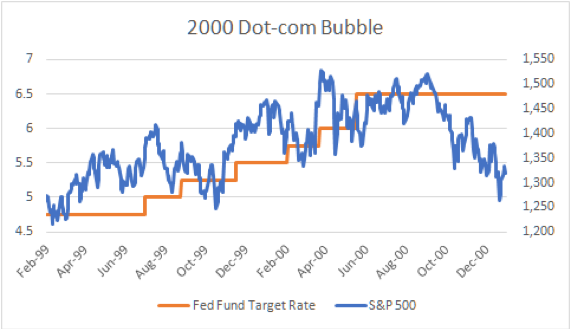
\includegraphics[width=1\linewidth]{pic1} 

}

\caption{Influence of Federal Reserve rate hike on S\&P500}\label{fig:pic1}
\end{figure}

\begin{figure}

{\centering 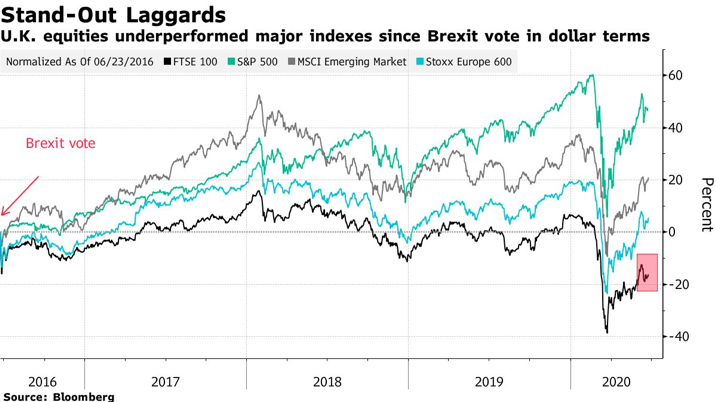
\includegraphics[width=1\linewidth]{pic2} 

}

\caption{ Influence of Brexit on uk stocks}\label{fig:pic2}
\end{figure}

\end{document}
